% ====================================================================
%+
% SECTION NAME:
%    wl.tex
%
% CHAPTER:
%    cosmology.tex
%
% ELEVATOR PITCH:
%-
% ====================================================================

\newcommand{\red}[1]{\textcolor{red}{#1}}

\clearpage
\section{Weak Lensing}
\def\secname{wl}\label{sec:\secname}

\credit{jmeyers314},
\credit{tonytyson}.

Much of LSST cosmology may be limited by systematic rather than statistical
errors.  This is especially true of weak gravitational lensing, which relies on
very accurate (\ie low bias), estimates of the shear of large ensembles of
galaxies. Measurements of the noisy shapes of many galaxies, and high
signal-to-noise measurements of PSF calibration stars are made.   Even though
the shot noise of the shape of an individual galaxy is very large, any small
shear bias could accumulate over many such galaxies.  As outlined in the SRD,
uniformity of seeing in the bands used for weak lensing and special observing
strategies are required in order to reduce additive and multiplicative shear
systematics.

Achieving the ultimate sensitivity of the LSST to weak lensing science places
stringent requirements on our ability to accurately estimate galaxy shapes and
redshifts, which in turn demands precise and accurate knowledge of the point
spread function, astrometry, and photometry.  These measurements are influenced
by the interaction of light with the Earth's atmosphere, the telescope optics,
and the CCD sensors.  Systematics in the shear are introduced in each case.
Observing strategies have been developed for suppressing these systematics in
current lensing surveys, such as the Deep Lens
Survey\footnote{\url{dls.physics.ucdavis.edu}}.  These and new methods will be
applied to the LSST survey.

To leading order, we can express the effect of shear systematics in the observed
shear $\gamma^\mathrm{obs}_i$ as a small linear perturbation of the true shear
$\gamma_i$,

$$ \gamma_i^\mathrm{obs} = (1+m_i) \gamma_i + c_i, $$

where $m_i$ is the multiplicative and $c_i$ is the additive systematic in the
ith shear component.  These systematics have contributions from the atmosphere
and the detector+optics.  Systematic errors in modeling the PSF from images of
stars and in interpolating the PSF from the positions of stars to the positions of
galaxies propagate to systematic errors in the galaxy shear.  To leading order, the
PSF contributions to the additive systematic are a linear function of the PSF
ellipticity.  The best observing strategies cause the average PSF ellipticity at a
given point (over all exposures) to average towards zero.

From the LSST SRD requirements on residual systematics in the galaxy shear-shear
correlation function one can specify the level of residual shear systematics at
which statistical uncertainties become subdominant.  Over the sample of 3-4
billion galaxies, the shear systematics must be below 3 parts in 10,000 for
additive shear $|c|$, and 3 parts in 1000 for multiplicative shear $|m|$.  Each
visit to a sky patch encounters these systematics.  In particular, each re-visit
to a given field generates the same CCD-based additive shear systematic.  Some
observing strategies can effectively randomize these over all visits to a field.
It is important to note that the full survey shear-shear correlation error due
to these systematics is expected to be no better than the corresponding
systematic in any given field after all re-visits to that field. This is because
the useful angular scales in cosmic shear are less than a field radius of
several degrees, and the systematics floor in shear-shear correlation is set
therefore by the floor in any one typical field.  Below we discuss the observing
strategies for suppressing shear systematics and metrics for their success.


\subsection{Target Selection}

Image quality must be uniformly good in the bands used for weak lensing shear.
These will be mainly the $r$ and $i$ bands, though it is possible that the $z$
band will also be used for shear measurement.  The decision on which field to
observe next must be based mainly on its weak lensing priority \citep[Sec 3.1
and Figure 14.4]{2009arXiv0912.0201L}.  Depending on the current weather and
seeing, the scheduler will have a list of priorities for next-field, based on
prior history of coverage.  The relevant parameters are seeing, depth, and
camera rotation angle with respect to North and to zenith. Nearby fields in need
of coverage in these bands should be given high priority if the seeing is better
than some specified value, likely 0.7 arcsec FWHM \citep[Sec
14.5.2]{2009arXiv0912.0201L}.

\subsection{Target Measurements}

It is expected that even after optimization of camera optics and electronics,
systematic image shape errors will be associated with the orientation of the
camera focal plane.  Using data from vendor CCDs, simulations of LSST observing
have shown that a combination of x-y dithering on the sky and pipeline
processing with pixel re-map (to cancel much of the CCD frame fixed distortions)
can get well within a factor of ten of the goal for shear systematics residuals.
Simulations which add camera angle dithering show that the residual shear
systematics goal can be achieved in fields with relatively uniform seeing
history \citep{Jee&Tyson2011}.  To average down the PSF systematics over many
re-visits we benefit from uniformly distributed image quality over the ensemble.
A non-uniform history in some field can be addressed by the scheduler taking
that into account for the offending rotation angle(s) in the history of prior
visits.

Thus shear systematics will be reduced by randomization of the orientation of
the camera with respect to the sky.  This is represented by the parameter
RotSkyPos, defined as the angle between the $+y$ camera direction and North.  We
can construct diagnostic metrics that quantify the uniformity of its
distribution at each sky position.  Given the spin 2 symmetry of shear, the
optimal strategy for shear systematics will be to aim for uniformity of
RotSkyPos mod $\pi$, since angles separated by $\pi$ radians are degenerate.

Similarly, the telescope optics may harbor systematic aberrations, and these
also could be mitigated by recording images with a uniform distribution of
parallactic angle, which is the angle between North and zenith for a given field
observation.  Differential chromatic refraction (DCR) effects will also be
mitigated by varying the parallactic angle, though the exact relationship is
complex since the parallactic angle sets both the DCR magnitude and direction
for a given observation.  Re-visits to a given field should be distributed over
parallactic angles (or equivalently, hour angles), consistent with airmass and
seeing limits.  Note that wide hour angle coverage for a given field will also
be helpful in order to efficiently achieve full 180 deg coverage in CCD sky
angle.

As argued below, survey depth is more important than survey area early in the
survey.  Uniformity of depth is important, but less so than uniformity in camera
rotator shear suppression.  Simulations have shown that for the Gold sample of
galaxies, uniformity at the 0.2 mag level in limiting magnitude produces little
shear bias.  The largest effect comes from bias in weak lensing magnification
tomography \citet{Morrison2012}.  This is important in the joint analysis of
LSST multi probes of cosmology.  Trends in survey depth can also propagate to
trends in photometric redshift.  These trends must be understood, if not
minimized.


\subsection{Metrics}

For characterizing the isotropy of rotational sampling, both for rotSkyPos and
the parallactic angle, we investigate two metrics: the AngularSpreadMetric and
the KuiperMetric.  The AngularSpreadMetric characterizes the balance of a set of
angular values, in the sense that opposing angles, those separated by $\pi$
radians, have zero contribution to the AngularSpread.  The Kuiper statistic,
which is related to the well known Kolmogorov-Smirnov statistic, characterizes
the departure of a distribution from uniform, but with the added quality of
being invariant under cyclic transformations of the input set of angles.

The AngularSpread metric is computed as follows:  Given a set of angles
$\{\theta\}_{i=1, ..., N}$, map these angles onto a unit circle: $(x_i, y_i) =
(\cos \theta_i, \sin \theta_i)$, and find the 2D centroid: $(\bar{x}, \bar{y}) =
\frac{1}{N} (\sum_i x_i, \sum_i y_i)$.  The AngularSpread is the distance of the
2D centroid from the unit circle: $\mathrm{AngularSpread} = 1 - \sqrt{\bar{x}^2 +
\bar{y}^2}$.  An AngularSpread of 1 therefore corresponds to a perfectly
balanced distribution, in which the averages of both $\cos \theta$ and $\sin
\theta$ are zero, while an AngularSpread of 0 indicates a maximally anisotropic
distribution in which every angle is identical: $\theta_i = \mathrm{const}$.  As
mentioned above, weak lensing shear systematics cancel to first order when those
systematics are separated not by an angle of $\pi$ radians on the sky, but by an
angle of $\pi/2$ radians (i.e., the difference in shear \emph{phase} is $\pi$
radians).  To incorporate this spin-2 nature of shear systematics is simple, we
just multiply each angle $\theta_i$ (either RotSkyPos or the parallactic angle)
by 2 before applying the AngularSpread metric, so that, for example, pairs of
angles separated by $\pi/2$ radians on the sky are separated by $\pi$ radians in
shear phase and correctly cancel.  See \autoref{fig:angularSpread} and caption for
an example of how the AngularSpread metric is used for weak lensing.

\begin{figure}
\centering
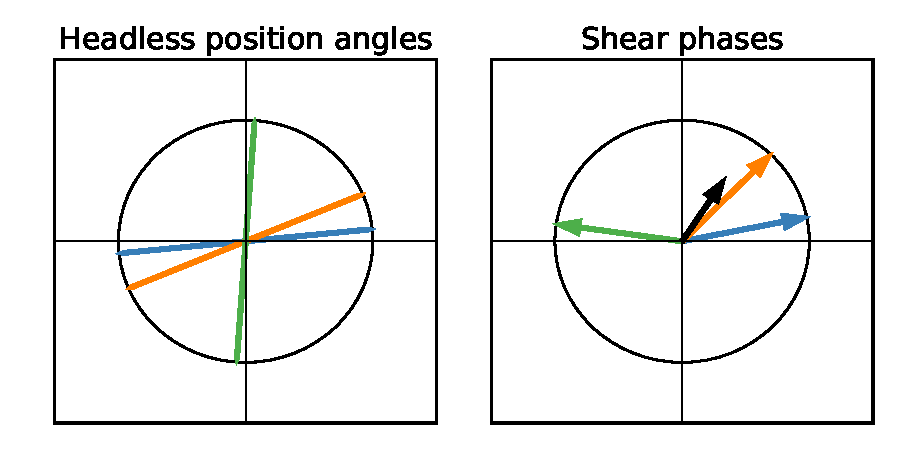
\includegraphics[width=\linewidth]{figs/WL/angularSpread.pdf}
\caption{Demonstration of AngularSpread metric.  \textbf{Left:} Three position
angles are indicated on a unit circle, using headless vectors since shear
systematics are invariant to 180-degree rotations.  \textbf{Right:} The
corresponding shear phases, which are twice the position angles, on a unit circle.
The black arrow indicates the 2D centroid of the 2D shear phases.  The
AngularSpread metric is the distance from the tip of this black arrow to the unit
circle.  Note that the blue and green position angle symbols, which are separated
by nearly 90-degrees and hence produce nearly opposing shear systematics, correspond
to blue and green shear phase vectors separated by nearly 180-degrees and hence
nearly cancel geometrically in the computation of the AngularSpread.}
\label{fig:angularSpread}
\end{figure}

% \begin{figure}
% \centering\includegraphics[width=\linewidth]{figs/enigma1189RmsAnglerotSkyPosugrizybandallpropsOPSIComboHistogram.png}
% \caption{The relative angle of the detector plane with respect to the sky, RotSkyPos, as a histogram showing the number of fields vs. rms of the parameter.}
% \label{RotSkyPos}
% \end{figure}


While the AngularSpread metric does a good job at characterizing the balance of
a distribution defined on a circle, it does not directly address the {\emph
{uniformity}} of said distribution.  For instance, the AngularSpread of the
angles $\{0, 0, 0, 0, \pi, \pi, \pi, \pi\}$ is zero, but the distribution is far
from uniform.  The Kolmogorov-Smirnov (KS) test is well known for investigating
whether a set of data are consistent with a given distribution.  The KS
statistic, off which the KS test is based, is defined as the maximum absolute
difference in the empirical cumulative distribution function (CDF) of the data
and the CDF of the distribution being tested.  The Kuiper statistic is a slight
modification of the KS statistic, defined as the sum of the maximum difference
and absolute minimum (maximally negative) difference between the empirical and
test CDFs.  This modification is convenient for characterizing distributions
defined on a circle, since it makes the statistic invariant under rotations of
the data.  The larger the Kuiper test statistic (which ranges between 0 and 1),
the larger the difference between the empirical distribution and the test
distribution.  To incorporate the spin-2 nature of shear systematics in the
Kuiper statistic, we map the values $\theta_i \rightarrow \theta_i \mod \pi$ and
compare to the uniform distribution between 0 and $\pi$.

The above metrics focus on the suppression of additive shear systematics.
Minimizing multiplicative shear systematics, and in particular estimating its
spatial variation is also important.  If the depth or average seeing are very
heterogeneous in their variation across the sky, then any multiplicative biases
that have to be corrected in the data analysis will have severe spatial
dependence. Homogeneity of depth and seeing certainly helps, and that is an
observing strategy question as discussed above.  A specific metric for
multiplicative systematics would be useful in our next \OpSim runs.  A useful
metric to be applied to full observing simulations is the mean ratio (and
spatial variance) of observed vs simulated shear amplitudes over a large sample
vs z-bins.  Since {\it Multi-Fit} joint star-galaxy fits to individual visits
will be used for data analysis, these PSF effects will be inherited for each
exposure and over that full field in a properly weighted fashion.  Other science
cases value uniformity of image quality as well, and this type of metric may be
applied during observing.


\subsection{\OpSim Analysis}

The distribution of AngularSpread for $2 \times$ rotSkyPos is shown in
\autoref{fig:WL_AngularSpread_rotSkyPos} for the latest baseline \OpSim run,
\opsimdbref{db:baseCadence}.  The left panel shows a sky map for the i-band (in this and the
following figures, the sky maps vary only minimally between the two principal
lensing filters, $r$ and $i$), while the right panel shows a histogram of values
for each LSST filter.  The distribution of the Kuiper statistic for rotSkyPos
mod $\pi$ is similarly shown in \autoref{fig:WL_Kuiper_rotSkyPos}.

While we do not currently have a method to quantitatively connect the
distribution of rotSkyPos to cosmological systematics, these figures appear to
indicate that rotSkyPos is already being well sampled in current simulations due
to the rotator tracking the sky during exposures, being subject to cable wrap
limits, and occasionally resetting to 0-degrees for filter changes.

\citet{Jee&Tyson2011} did a study of the shear residual systematics due to known
LSST CCD brighter-fatter anisotropy in 100 revisits to a single field with
random angular orientations and seeing sampled from the expected distribution.
The Data Management (DM) pipeline will use a model of the charge transport in
the CCD to re-map pixel shapes, sizes, and areas in pixel level data processing.
The needed factor of 10 suppression of the CCD-based shear systematic residuals
(post pixel remap pipeline correction) was obtained, reaching the SRD floor on
cosmic shear systematics (presented at weak lensing systematics workshop, Dec
2015)\footnote{\url{https://indico.bnl.gov/conferenceDisplay.py?confId=1604}}.
Of course, the requirements for spatial dithering for shear systematics
residuals depend on the precision of the pixel processing for removal of the CCD
based additive shear systematic.  We assume that this pixel level remap in the
DM pipeline cannot correct to better than 3 times the rms errors in the lab
tests for dynamic and static CCD systematics.

The distribution of parallactic angles is similarly shown in
\autoref{fig:WL_AngularSpread_ParallacticAngle} and
\autoref{fig:WL_Kuiper_ParallacticAngle}.  These figures show significantly less
isotropy and significantly more structure across the survey footprint than those
for rotSkyPos, likely due to the fact that, unlike rotSkyPos, the parallactic
angle is independent of the camera rotator position.  Hence, the parallactic
angle is more tightly constrained by geometry than rotSkyPos.  In fact, the only
mechanism by which the parallactic angle varies for a given field is through
variations in the hour angle at which that field is observed.

% \begin{figure}
% \centering\includegraphics[width=\linewidth]{figs/enigma1189RmsAnglerotSkyPosugrizybandallpropsOPSIComboHistogram.png}
% \caption{The relative angle of the detector plane with respect to the sky, RotSkyPos, as a histogram showing the number of fields vs. rms of the parameter.}
% \label{RotSkyPos}
% \end{figure}

% The distribution of rms values by filter is shown in
% \autoref{RotSkyPos} for the current candidate baseline simulation,
% enigma\_1189.  As shown, the rms values cluster around the value 1
% radian,  with typical values 1 +- 0.3 radian.  This compares to a
% completely uniform distribution over the half circle with an rms of
% 1.14.  As mentioned above, uniformity in cosine squared is the goal.
% Simulated observing of 100 visits to a field show this will produce
% a factor of 10 decrease in CCD-based shear systematics such as edge
% effects and the brighter-fatter x-y anisotropy.




\newcommand\plottwo[2]{{%
\typeout{Plottwo included the files #1 #2}
\centering
\leavevmode
\includegraphics*[width=0.45\columnwidth]{#1}%
\hfil
\includegraphics*[width=0.45\columnwidth]{#2}%
}}%


%  rotSkyPos metrics

\begin{figure}[tbh!]
\plottwo{figs/WL/minion_1016_AngularSpread_rotSkyPos_propID_54_and_i_HEAL_SkyMap.pdf}
        {figs/WL/minion_1016_AngularSpread_rotSkyPos_u_g_r_i_z_y_propID_54_HEAL_ComboHistogram.pdf}
\caption{\textbf{Left:} Sky map showing the distribution of the AngularSpread
    metric applied to the angle $2 \times$ rotSkyPos, where rotSkyPos is the
    angle between the $+y$ camera direction and North, and the factor of 2
    takes into account the degeneracy of angles separated by $\pi$ radians for
    spin-2 shear systematics.  An AngularSpread of 0 indicates a maximally
    anisotropic distribution (all visits have the same angle), while an
    AngularSpread of 1 indicates that visits are maximally balanced (the mean of
    $\cos \theta$ and $\sin \theta$ are both 0.) For the complete definition of
    the AngularSpread metric, please see the text.  To leading order, shear
    systematics permanently imprinted on the camera cancel when AngularSpread =
    1.  \textbf{Right:} Distribution of the AngularSpread metric applied to
    $2 \times$ rotSkyPos for all six LSST filters.}
\label{fig:WL_AngularSpread_rotSkyPos}
\end{figure}

\begin{figure}[tbh!]
\plottwo{figs/WL/minion_1016_Kuiper_rotSkyPos_propID_54_and_i_HEAL_SkyMap.pdf}
        {figs/WL/minion_1016_Kuiper_rotSkyPos_u_g_r_i_z_y_propID_54_HEAL_ComboHistogram.pdf}
\caption{\textbf{Left:} Sky map showing the distribution of the Kuiper metric
    (see text for definition) applied to the angle rotSkyPos mod $\pi$.  A
    Kuiper value of 0 indicates an isotropic distribution of angles (mod $\pi$),
    while a Kuiper value of 1 indicates a maximally anisotropic distribution.
    \textbf{Right:} Distribution of the Kuiper metric applied to (rotSkyPos mod
    $\pi$) for all six LSST filters.}
\label{fig:WL_Kuiper_rotSkyPos}
\end{figure}

%  ParallacticAngle metrics

\begin{figure}[tbh!]
\plottwo{figs/WL/minion_1016_AngularSpread_ParallacticAngle_propID_54_and_i_HEAL_SkyMap.pdf}
        {figs/WL/minion_1016_AngularSpread_ParallacticAngle_u_g_r_i_z_y_propID_54_HEAL_ComboHistogram.pdf}
\caption{Same as Fig. \ref{fig:WL_AngularSpread_rotSkyPos}, but for the
    parallactic angle (the angle between North and zenith) instead of rotSkyPos.
    The isotropy of the parallactic angle affects the impact of shear
    systematics due to telescope aberrations and differential chromatic
    refraction.}
\label{fig:WL_AngularSpread_ParallacticAngle}
\end{figure}

\begin{figure}[tbh!]
\plottwo{figs/WL/minion_1016_Kuiper_ParallacticAngle_propID_54_and_i_HEAL_SkyMap.pdf}
        {figs/WL/minion_1016_Kuiper_ParallacticAngle_u_g_r_i_z_y_propID_54_HEAL_ComboHistogram.pdf}
\caption{Same as Fig. \ref{fig:WL_Kuiper_rotSkyPos}, but for the parallactic
    angle instead of rotSkyPos.}
\label{fig:WL_Kuiper_ParallacticAngle}
\end{figure}


\subsection{Ancillary data}

Optimal observing strategy relies on the use of all relevant data, with current
and historical coverage per field.  Ancillary data, and auxiliary uses of the
science exposures, play an important role informing next-field strategy.  We can
use large scale patterns of distortions of the PSF over the 20,000 stars per
exposure for PSF regularization in the per-CCD PSF fitting.  In the per CCD
fits, there is a benefit to setting aside some stars for validation tests of PSF
extrapolation.  These data may be used as a metric for image quality and thus
the ranked value of an exposure for shear systematics removal.  Fields with poor
image quality rise to the top of the priority list for re-observing at that
camera angle.  In addition to using all the stars in a given visit, there is
useful information in the wavefront sensors and the guide CCDs that may be used
to regularize the PSF reconstruction in a visit.  We might read out guider CCDs
in different ways to better monitor the atmosphere.


\subsection{Deep vs Wide}

As outlined above, many revisits to each field spanning many RotSkyPos angles
aids the suppression of additive shear systematics.  For a given per-visit
exposure time this leads to a deep survey, due to the multitude of visits.
There are several advantages to a deep survey over a shallow-wide survey for
weak lensing science, especially for dark energy where a range of lens redshifts
is required to sample the growth of dark matter structure from low redshift to
redshift beyond 1.  A strategy question for LSST is whether to go wide first and
then deep, or the reverse.  There are actually several drivers for depth over
area, given fixed observing time and camera+telescope etendue.  Provided that
sufficient area is covered to overcome sample variance at lower redshifts and to
adequately cover the important angular scales, a deep observing strategy
maximizes the cosmological signal-to-noise ratio both by maximizing the signal
and minimizing the noise.

First, a deep survey strategy boosts the amplitude of the cosmic shear signals
due to the increased amplitude of the lensing kernel.  Given the same lens mass,
the amplitude of lensing signals is a simple function of the two distances:
observer-to-lens versus lens-to-source.  For example, when a lens is at $z =
0.5$, the shear for a source at $z = 1.1$ is nearly twice that at $z = 0.7$,
leading to a factor of 4 ratio in correlation function amplitudes.  Thus, a deep
survey can take advantage of the geometric effect of gravitational lensing more
efficiently.

Second, a deep survey strategy enables a longer redshift baseline to break
parameter degeneracies.  For example, shallower surveys with wider area are not
efficient in shrinking the length of the ``banana'' in the $\Omega_M$-$\sigma_8$
plane because of the $\sigma_8 \Omega_M^\alpha = \mathrm{const}$ degeneracy.
The deep strategy compensates for the loss of volume due to a reduced area by
extending the volume along the line of sight.

Third, deep surveys provide more useful galaxies per area.  This merit does not
entirely overlap with the second point.  In addition to new sources at higher
redshift, the fainter limiting magnitude enables detection of fainter galaxies
at a given redshift and better signal-to-noise ratio.  This argument requires
that photometric redshifts of this population of galaxies is as well-calibrated
as those at lower redshift.  This may be done via cross-correlation with sample
low-z galaxies.  Needless to say, the increased source density reduces the
impact of shape noise caused by intrinsic ellipticity dispersion.

Fourth, it mitigates the effects of intrinsic alignments (IA), an important
theoretical systematic in precision cosmic shear.  Current studies
\citep{Heymans2013} indicate that IA effects are dominated by luminous red
galaxies (LRGs).  Because a deep survey can access fainter galaxies, the net IA
systematic decreases because the fraction of the LRGs decreases at fainter
limiting magnitude.  Using the approach of \citet{Joachimi2011}, at $z = 0.5$
the amplitude of the IA power spectrum is reduced by a factor of two for an
increase in the limiting $r$ magnitude from 24 to 27 mag.

For cosmic shear the volume at $\sim 5$ arcminute to several degree scales and
over a wide range of redshift is most important.  Once a fair sampling of
“cosmic variance” is achieved the depth matters most, because of the z-width of
the lensing kernel.  With fixed survey duration on a camera+telescope of fixed
etendue, it is better to prioritize depth in order to maximize the weak lensing
cosmological signal-to-noise ratio.  In particular, for the LSST survey it would
be helpful to have several widely spaced deep drilling fields done early and
deeper than the main survey, in order to explore detailed observing strategies --
particularly the angle dither scheme.  Deep drilling data is useful to a variety
of LSST science drivers, including Bayesian analyses.  By the same reasoning, it
would be important to cover a significant area [perhaps 2000 sq. deg] to full
depth during the first year of the survey.  This would allow full assessment of
systematics, and could be chosen to overlap the WFIRST footprint.

Metrics for reaching the SRD goals for WL related science are needed. Long
before LSST is on the sky such metrics can be applied to realistic simulations
of LSST observing, in order to inform the scheduler proposal ranking algorithm.
One metric is the sample variance in cosmic shear in 10 sq. deg DD fields versus
that, for say, 1000 sq. deg.  A related systematics metric would be the
suppression of additive PSF systematic residuals in 1000 sq. deg worth of
pointings over the sky, normalized by that in one field visited 100 times. These
important simulations will be enabled by the deep-wide full cosmological
simulation deliverables in DESC Data Challenges 2 and 3, together with \OpSim
runs.


\subsection{Discussion}

The RotSkyPos metrics show that the majority of fields have good randomization
of detector angles projected on the sky.  The randomization of parallactic
angles is less successful, though this is to be expected due to fewer knobs
available to adjust the parallactic angle of observations of a given field.  In
both cases, however, a significant fraction of fields show metric values lower
than expected for a uniform distribution.  Regardless of the \emph{per field}
criterion adopted, it is desirable to avoid the incidence of individual
discrepant fields.  The recommended criterion for randomization of RotSkyPos and
parallactic angle is not the behavior of the majority of the fields, but of the
minority with the least random behavior -- the number of non-random fields
should be minimized.

It is certain that actively controlling the statistics of RotSkyPos will require
additional slewing of the camera rotator.  At present, the operations plan is to
only slew (beyond that required to track the sky during exposures) when
necessary to prepare for a filter change -- that could be estimated at the
equivalent of $\simeq 3$ complete rotations per night.  To engage the rotator by
up to $\simeq 30$ degrees per visit would require $\simeq 300$ complete
rotations per night - an upper limit to the additional rotations, but one which might be approached by a requirement for
rigorous distribution over relatively short timescales.  On the other hand, a very significant improvement
in distribution could be achieved by simply introducing a constrained randomized rotator
offset after each filter change, with little or possibly no loss in observing efficiency.
Guidance is needed from simulations for the randomization requirement(s), and from science strategy
for the time scale over which it must be achieved.

Increasing the isotropy of the parallactic angle is trickier, since the
parallactic angle is only affected by the hour angle of observations (for a
given field).  It may be possible, however, to adjust the scheduler cost
function to better favor parallactic angle isotropy.

In summary, image quality weighted randomization of RotSkyPos is required at
10-20\% scatter in image quality over the sample of visits (2015 simulation
mentioned above).  Randomization of parallactic angle is also desired, but a
requirement is yet to be determined.  Interestingly, there is an excellent
opportunity to combine these two randomizations in an efficient observing
strategy which actually minimizes the number of camera rotations.  Re-visits to
a field over a range of hour angles and with camera rotations assures full 180
degree range coverage for CCD coordinates relative to sky.  A metric for this
can be written and run with \OpSim to explore optimization, including minimizing
camera rotations.

\subsection{Conclusions}

Randomization of camera angle covering 180 deg can effectively suppress
residual shear systematics remaining after DM pipeline first-order
correction.   More simulations are required, using intelligent
dithering, in order to assess the efficiency and the remaining WL shear
systematics.


We can now provide answers to the ten questions posed in %
\autoref{sec:intro:evaluation:caseConclusions}:

\begin{description}

\item[Q1:] {\it Does the science case place any constraints on the
tradeoff between the sky coverage and coadded depth? For example, should
the sky coverage be maximized (to $\sim$30,000 deg$^2$, as e.g., in
Pan-STARRS) or the number of detected galaxies (the current baseline 
of 18,000 deg$^2$)?}

\item[A1:] On the scale of thousands of sq.deg, the WL signal and
control of systematics is enhanced by deeper (larger cosmological
volume) rather than wider surveying. These considerations led to the
18,000 sq.deg per ten years baseline.

\item[Q2:] {\it Does the science case place any constraints on the
tradeoff between uniformity of sampling and frequency of  sampling? For
example, a rolling cadence can provide enhanced sample rates over a part
of the survey or the entire survey for a designated time at the cost of
reduced sample rate the rest of the time (while maintaining the nominal
total visit counts).}

\item[A2:] WL is generally agnostic on this issue. Total good IQ x depth
is most important, and this might benefit from rolling cadences if the
mean airmass is lower, resulting in a higher IQ.


\item[Q3:] {\it Does the science case place any constraints on the
tradeoff between the single-visit depth and the number of visits
(especially in the $u$-band where longer exposures would minimize the
impact of the readout noise)?}

\item[A3:] 30-sec or longer u band exposures will help S/N.

\item[Q4:] {\it Does the science case place any constraints on the
Galactic plane coverage (spatial coverage, temporal sampling, visits per
band)?}

\item[A4:] WL ugrizy imaging must avoid low Galactic latitudes due to
stellar crowding, bright stars, and dust. Data at low latitudes will not
be used for WL.

\item[Q5:] {\it Does the science case place any constraints on the
fraction of observing time allocated to each band?}

\item[A5:] This depends on the relative system throughput vs wavelength.
For the case of high u band QE CCDs, approximately u10\%, g10\%, r22\%,
i22\%, z18\%, y18\%. The comes from 80, 80, 184, 184, 160, 160 ugrizy
30-sec visits per 9.6 sq.deg fields over 18,000 sq.deg per ten years --
from the SRD, driven by required low surface brightness shear
measurement and the needed S/N for photo-z for the gold sample of
galaxies. The longer integrations at longer wavelengths is due to the
red color of the sky background.

\item[Q6:] {\it Does the science case place any constraints on the
cadence for deep drilling fields?}

\item[A6:] It will be helpful if the individual exposure times in all
bands are similar to the main survey. A long series of exposures in each
filter would be good. Dithering in x-y-theta between exposures using
“intelligent dithering” is needed in order to detect low level
systematics and to help calibrate the main survey galaxy blending.
Emphasis on excellent seeing is important. Spreading the DD observing
over many half nights, maximizing the HA coverage, will be needed.

\item[Q7:] {\it Assuming two visits per night, would the science case
benefit if they are obtained in the same band or not?}

\item[A7:] Not necessarily. In fact, occasional back-to back gr
exposures help calibrate systematics from chromatic refraction.

\item[Q8:] {\it Will the case science benefit from a special cadence
prescription during commissioning or early in the survey, such as:
acquiring a full 10-year count of visits for a small area (either in all
the bands or in a  selected set); a greatly enhanced cadence for a small
area?}

\item[A8:] Yes, ugrizy full depth over at least 1000 sq.deg. Suppression
of WL systematics will depend on early detection of issues. This, and
the development and validation of MultiFit pipline, shear measurement
algorithms, cosmological analysis algorithms, and associated covariances
will rely on early deep surveying of a few thousand square degrees. This
also benefits co-analysis with WFIRST or Euclid data.

\item[Q9:] {\it Does the science case place any constraints on the
sampling of observing conditions (e.g., seeing, dark sky, airmass),
possibly as a function of band, etc.?}

\item[A9:] WL benefits significantly from good uniform seeing, IQ, and
depth in the r and I bands. For example, imaging in the r and i bands in
seeing worse than 1 arcsec is not productive, and revisits to that field
should await better seeing. The associated photo-z relies on uniform
depth spatially. This means low airmass.

\item[Q10:] {\it Does the case have science drivers that would require
real-time exposure time optimization to obtain nearly constant
single-visit limiting depth?}

\item[A10:] Yes. Uniform residual shear is even more important than
depth. Dithering in x-y-theta between exposures using “intelligent
dithering” is needed in order to detect low level systematics and to
help calibrate the main survey galaxy blending. In intelligent dithering
the scheduler is aware of the past history of the IQ in that field in
the two bands used for WL shear (nominally r and i). The algorithm tries
to uniformly sample camera angles relative to north with uniformly good
IQ. Rotation angles of previous poor IQ visits need to be repeated.

\end{description}


% The RotSkyPos metric analysis shows that the majority of fields have a
% good randomization of detector angles projected on the sky.
%
% There are some limitations to this observation.
%
% %First, we do not have at present a quantitative requirement for
% %randomization of this parameter.  In future development of weak
% %lensing analysis, a criterion should be developed.
%
% A significant fraction of fields  have median values that are
% lower or higher than expected for a random distribution, with some far
% from uniformly distributed.  Regardless of the $per field$ criterion,
% it is desirable to avoid the incidence of individual discrepant
% fields.
%
% The recommended criterion for randomization of RotSkyPos is not the
% behavior of the majority of the fields, but of the minority with the
% least random behavior.  The number of non-random fields should be
% minimized.  A recommended metric is the count of fields with median
% RMS less then 0.8 or greater than 1.5 radians (these values to be
% reviewed again as additional experience is gained with additional
% OpSim schedule simulations and weak lensing analysis.)
%
% It is certain that actively controlling the statistics of RotSkyPos
% will require additional slewing of the camera rotator.  At present,
% the operations plan is to only slew when necessary to prepare for a
% filter change - that could be estimated at the equivalent of $\simeq
% 3$ complete rotations per day.  \autoref{RotSkyPos} shows that to
% render the distribution completely uniform would require moving all
% observing angles an average of $\simeq 30$ degrees, or 300 complete
% rotations per night.  The timing of this has not been considered.
% Whether or not this uniformity could be achieved with less slew time
% if implemented in scheduling remains to be demonstrated.
%
% A similar metric for RotTelPos should be developed.
